\documentclass[12pt, a4paper]{scrartcl}

% CONFIG
\newcommand{\exptitle}{Farady- und Pockelseffekt}       % long name of experiment 
\newcommand{\exptitleshort}{FarPock} % short name of experiment
\newcommand{\expdate}{24. und 25. September, 2014}           % date of experiment
\newcommand{\exptutor}{Florian Ki\ss}

% PACKAGES + MODIFICATIONS
\usepackage[ngerman]{babel} %standard language stuff
\usepackage[T1]{fontenc}
\usepackage[utf8]{inputenc}
\usepackage{textgreek}

\usepackage[fleqn]{amsmath}  % math
\usepackage{amssymb}

\usepackage{graphicx} %graphics
\usepackage{float} 

\usepackage[automark,headsepline]{scrlayer-scrpage} %headings
\pagestyle{scrheadings}
\ihead{\exptitleshort}
\ohead{\pagemark}
\cfoot{}

\usepackage{hyperref}
\hypersetup{
    unicode=true,          % non-Latin characters in Acrobat’s bookmarks
    pdftoolbar=true,       % show Acrobat’s toolbar?
    pdfmenubar=true,       % show Acrobat’s menu?
    pdffitwindow=false,    % window fit to page when opened
    pdfstartview={FitH},   % fits the width of the page to the window
    pdfnewwindow=true,     % links in new window
    colorlinks=true,       % false: boxed links; true: colored links
    linkcolor=blue,       % color of internal links (change box color with linkbordercolor)
    citecolor=green,       % color of links to bibliography
    filecolor=magenta,     % color of file links
    urlcolor=blue          % color of external links
}

\usepackage[labelfont=bf]{caption} % bold captions

\usepackage{chngcntr} % change behaviour of counters in different environments
\counterwithin{figure}{section}  % number figures per section
\numberwithin{equation}{section} % number equations per section
\numberwithin{table}{section}    % number tables per section

\usepackage{enumerate} % better way to config enumerates

\setcounter{tocdepth}{3} % table of contents depth

\setlength{\parindent}{0pt} % no indent on new paragraph

\usepackage{pdfpages} % include pdf files

\usepackage[nottoc,numbib]{tocbibind} % bibliography in TOC

% NEW COMMANDS
\newcommand{\difd}{\mathrm{d}}
\newcommand{\abs}[1]{\left|#1\right|}
\newcommand{\refeq}[1]{\overset{\text{\eqref{#1}}}{=}}

% DOCUMENT SETTINGS

\title{\exptitle}
\subtitle{Fortgeschrittenen-Praktikum 1}
\author{Moritz Bitterling und Benjamin Rottler \\ Universität Freiburg}
\date{\expdate}

% DOCUMENT
\begin{document}

\hypersetup{pageanchor=false} %stop page numbering (hyperref) to prevent for double page numers
\newcommand{\HRule}{\rule{\linewidth}{0.5mm}}
\begin{titlepage}
\begin{center}
  \textsc{\Large Fortgeschrittenen Praktikum I}\\[0.5cm]
  \HRule \\[0.4cm]
  { \huge \bfseries \exptitle}\\
  \HRule \\[1.5cm]
  
  \begin{minipage}{0.4\textwidth}
    \begin{flushleft} \large
      Moritz \\ \textsc{Bittlering}
    \end{flushleft}
  \end{minipage}
  \hfill
  \begin{minipage}{0.4\textwidth}
    \begin{flushright} \large
      Benjamin \\ \textsc{Rottler}
    \end{flushright}
  \end{minipage}
  \\[1cm]
  \large 
  \emph{Datum der Veruchsdurchführung:} \expdate  \\
  \emph{Betreuer}: Riccardo \textsc{Mori} \\[3cm]
  \includegraphics[height=8cm]{../../img/logo_uni.pdf}
  \vfill
  \normalsize
  \textsc{Institut für Mathematik und Physik} \\
  \textsc{Albert-Ludwigs-Universität} \\
  \textsc{Freiburg im Breisgau}
\end{center}
\end{titlepage}
\thispagestyle{empty}

\newpage
Alle Berechnungen in diesem Protokoll wurden entweder unter Python 2.7 mit Hilfe folgender Programmbibliotheken
\begin{itemize}
  \item PyROOT (\url{http://root.cern.ch/drupal/content/pyroot})
  \item NumPy (\url{http://www.numpy.org/})
\end{itemize}
oder Mahtematica 9 und 10 durchgeführt. \\
Die Graphiken wurden mit Inkscape (\url{http://www.inkscape.org}) gezeichnet.\\[\baselineskip]
Alle Python-Skripte, \LaTeX-Skripte und SVG-Graphiken können online unter \\
\url{https://github.com/Bigben37/FP1/tree/master/0924-FarPock} abgerufen werden.
\thispagestyle{empty}

\newpage
\tableofcontents
\thispagestyle{empty}

\newpage
\hypersetup{pageanchor=true} %start page numbering again
\setcounter{page}{1} %set to page 1

\section{Versuchsziel}
Im Halbleiter-Versuch werden in drei verschieden Versuchsteilen unterschiedliche
halbleiterphysikalische Effekte untersucht:
Mit einer Transmissions- und Absorptionsmessung werden die \emph{Bandlücken} von Germanium und Silizium bestimmt.
Beim Haynes-Shockley-Experiment erhält man Informationen über die \emph{Mobilität}, \emph{Diffusionskonstante} und
\emph{mittlere Lebensdauer} der Elektronen im Leitungsband von Germanium.
Außerdem wird mit dotierten Halbleitern das \emph{Energiespektrum} von radioaktiven Proben aufgenommen. 

\section{Pockels-Effekt}
\subsection{Physikalische Grundlagen}
Die Gleichungen und Erklärungen dieses Kapitels beruhen auf \cite{herrmann}.
\subsubsection{Elektrooptischer Effekt}
Die elektrische Flussdichte $D$ ändert sich, wenn man ein äußeres elektrisches Feld anlegt. Diese Veränderung wird 
\emph{elektrooptischer Effekt} genannt und durch folgende Formel beschrieben:
\begin{equation}
\label{eq:eoeff}
  D = a \cdot E + b \cdot E^2 + c \cdot E^3 + \ldots
\end{equation}
Die Dielektrizitätskonstante\footnote{Wie man hier sieht, ist die Dielektrizitätskonstante keine Konstante, der Name hat historischen Ursprung.} 
$\epsilon$ lässt sich durch Differentiation von $D$ nach $E$ berechnen.
\begin{equation}
\label{eq:dielconst}
  \epsilon = \frac{\difd D}{\difd E} = a + 2 \cdot b \cdot E + 3 \cdot c \cdot E^2 + \ldots
\end{equation}
Der lineare elektrooptische Effekt oder \emph{Pockels-Effekt} tritt bei Kristallen ohne Symmetriezentrum auf, was zur Folge hat, dass 
der lineare Teil $2 \cdot b \cdot E$ nicht verschwindet. Der Einfluss von höheren Potenzen von $E$ ist sehr gering, da die Konstanten 
$b, c, \ldots$ sehr kleine Werte annehmen, und kommt nur bei sehr hohen elektrischen Feldstärken zum tragen. 
Für $b = 0$ und $c \neq 0$ spricht man vom \emph{Kerr-Effekt}. \\
Da der Brechungsindex $n$ von der Dielektrizitätskonstante abhängt, wirkt sich der Po"-ckels-Effekt auf die Brecheigenschaften des Kristalls aus.
\begin{equation}
  n = \sqrt{\epsilon \mu}
\end{equation}

\subsubsection{Doppelbrechung in Kristallen}
In einem optisch isotropen Medium ist die Lichtausbreitung unabhängig von der Ausbreitungsrichtung und Polarisation des Lichtes. Dies gilt bei 
einem optisch anisotropen Medium nicht mehr, man spricht von \emph{Doppelbrechung}. Bei optisch anisotropen Medien unterscheidet man zwischen 
optisch einachsigen und optisch zweiachsigen. Ja nach Typ gibt es eine oder zwei ausgezeichnete Richtungen, in denen ein Lichtstrahl für alle 
Polarisationen die gleiche Ausbreitungsgeschwindigkeit besitzt. \\
Man führt die Bezeichnung ordentlicher und außerordentlicher Strahl ein. Der ordentliche Strahl ist die Komponente des $E$-Feldes, die senkrecht 
auf dem Hauptschnitt (Ebene, die durch den $\vec{k}$-Vektor und die optische Achse des Kristalls aufgespannt wird) steht. Der außerordentliche 
Strahl liegt in der Ebene des Hauptschnitts.\\
Der Formalismus des Brechungsindex-Ellipsoids ist eine einfache Möglichkeit zur Beschreibung der Doppelbrechung. 
\begin{equation}
  \frac{x_1^2}{n_1^2 } +\frac{x_2^2}{n_2^2 } +\frac{x_3^2}{n_3^2 } = 1 
\end{equation}
Die Koordinaten $x_1, x_2, x_3$ spannen ein kartesisches Koordinatensystem auf. Mindestens eine Achse muss parallel zu einer kristallographischen 
Achse des Kristalls liegen. Die Brechungsindizes $n_1, n_2, n_3$ gelten für Licht, das sich parallel zu den entsprechenden Achsen ausbreitet. 
Kennt man das Brechungsindex-Ellipsoid, so kann man die unterschiedlichen Ausbreitungsrichtungen mit 
$v=\frac{c}{n}$ bestimmen. Die Form des Brechungsindex-Ellipsoid eines optisch isotropen Mediums ist eine Kugel, es verformt sich zu einer 
Ellipse bei einem anisotropen Medium.

\subsubsection{Konfiguration der Pockelszelle}
\paragraph{Bestimmung der Brechungsindizes}
In diesem Versuch wird eine Pockelszelle, die aus vier ADP\footnote{Ammoniumdihydrogenphosphat}-Kristallen mit einem $45^\circ Y$-Cut besteht, 
verwendet. Legt man an eine normale ADP-Zelle einen Spannung $E_1$ entlang der $x_1$ Achse an, so lautet das Indexellipsoid nach \cite{manual}:
\begin{equation}
  \frac{x_1^2}{n_1^2} + 2 \cdot r_{41} \cdot E_1 \cdot x_3 + \frac{x_2^2}{n_1^2} + \frac{x_3^2}{n_3^2} = 1
\end{equation}
mit $r_{41}$ als \emph{elektrooptischer Koeffizient}. Man erkennt, dass der Kristall optisch einachsig ist und die $x_3$-Achse die optische Achse ist. \\
Der $45^\circ Y$-Cut wird mit Hilfe einer Koordinatentransformation berücksichtigt:
\begin{equation}
  x_2 = \frac{1}{\sqrt{2}} \left( x_2' + x_3' \right), \qquad x_3 = \frac{1}{\sqrt{2}}(x_2' - x_3')
\end{equation}
Daraus folgt nach \cite{manual} für den Brechungsindex der $x_2'$-Achse:
\begin{equation}
  \label{eq:refindex:x2new}
  n_{x_2'} \approx n_x + \frac{1}{2} \cdot r_{41} \cdot E_1 \cdot n_x^3
\end{equation}
mit
\begin{equation}
  \label{eq:nxdef}
  \frac{1}{n_x^2} = \frac{1}{2} \left( \frac{1}{n_2^2} + \frac{1}{n_3^2} \right)
\end{equation}
\paragraph{Bestimmung der Phasenverschiebung}
Die ortsabhängige Amplitude des sich im Kristall ausbreitenden Lichts lässt sich mit
\begin{equation}
  A(x) = A_0 \cdot e^{ikx} = A_0 \cdot e^{i \varphi(x)}
\end{equation}
beschreiben. Mit der \emph{Dispersionsrelation} $\omega = v\cdot k$ und den Beziehungen $\omega = 2 \pi f$, $c = f \cdot \lambda$ 
und $v = \frac{c}{n}$ folgt für die Phase $\varphi$ der Welle.
\begin{equation}
  \varphi(x) = \frac{2 \pi}{\lambda} \cdot n \cdot x
\end{equation}
Es ergibt sich eine Phasendifferenz $\Delta \varphi$ in einem Kristall der Länge $l$ von
\begin{equation}
  \Delta \varphi = \frac{2 \pi}{\lambda} \cdot l \cdot \left( n_1 - n_{x_2'} \right) 
\end{equation}
Durch die Lage der optischen Achse laufen jetzt jedoch ordentlicher und außerordentlicher Strahl auseinander. Sie werden mit einem zweiten, 
um $180^\circ$ gedrehten ADP-Kristall wieder zusammengeführt. Die Phasendifferenz verdoppelt sich.
\begin{equation}
  \Delta \varphi = \frac{4 \pi}{\lambda} \cdot l \cdot \left( n_1 - n_{x_2'} \right) 
\end{equation}
Da der ADP-Kristall ein optisch einachsiger Kristall ist, besitzt er auch natürliche Doppelbrechung $n_1 - n_x$. Diese wird durch ein zweites 
Kristallpaar, das um $90^\circ$ gedreht ist ausgeglichen. Um Pockels-Effekt nicht auch aufzuheben, wird das zweite Paar mit invertierter Spannung 
betrieben. Dadurch verdoppelt sich die Phasendifferenz noch einmal. Es gilt also:
\begin{equation}
  \begin{split}
    \Delta \varphi &= \frac{8 \pi}{\lambda} \cdot l \cdot \left( n_1 - n_{x_2'} \right) \\
    &\refeq{eq:refindex:x2new} \frac{8 \pi}{\lambda} \cdot l \cdot \left( \underbrace{n_1 - n_x}_{=0} + \frac{1}{2} \cdot r_{41} \cdot E_1 \cdot n_x^3 \right) \\
    & = \frac{4 \pi}{\lambda} \cdot l \cdot r_{41} \cdot E_1 \cdot n_x^3  
  \end{split}
\end{equation}
Legt man nun die Halbwellenspannung $U_{\lambda/2}$ an, so beträgt die Phasendifferen gerade $\Delta \varphi = \pi$.
Unter Verwendung von $E=\frac{U_{\lambda/2}}{d}$ und \autoref{eq:nxdef} lässt sich der \emph{elektrooptische Koeffizient} $r_{41}$ folgendermaßen bestimmen:
\begin{equation}
  \label{eq:r41}
  r_{41} = \frac{\lambda \cdot d}{4 \cdot l \cdot U_{\lambda/2}} \sqrt{\frac{1}{2} \left( \frac{1}{n_1^2} + \frac{1}{n_3^2} \right) }^3
\end{equation}
mit $l$ Länge und $d$ Dicke (Kantenlänge) der Pockelszelle, sowie der Brechungsindizes $n_1$ und $n_3$.
\input{03_Aufbau_p}
\subsection{Versuchsdurchführung}
\subsubsection{Bestimmung der Halbwellenspannung mit einer Sägezahnspannung}
Um eine grobe Abschätzung der Halbwellenspannung zu bekommen,
wird im ersten Versuchsteil an die Pockelszelle das Sägezahnsignal angelegt.
Gleichzeitig wird mit dem Oszilloskop das Spannungssignal nach dem Verstärker der Photodiode gemessen.
Durch Drehen des Analysators wird dieses Signal so eingestellt,
dass die Amplitude maximal ist, aber kein \emph{Clipping} auftritt.
Die beiden Signale werden mit dem Computer aufgezeichnet.
Anschließend wird der Analysator für zwei weitere Messungen jeweils ein wenig weiter verdreht,
um eine eventuelle Amplitudenabhängigkeit der Halbwellenspannung zu identifizieren. 


\subsubsection{Bestimmung der Halbwellenspannung durch Periodenverdopplung eines Wechselsignals}

\paragraph{Ursache der Periodenverdopplung}
In diesem Versuchsteil wird die Halbwellenspannung mit einer genaueren Messmethode bestimmt:
Wenn ein Wechselsignal einer Gleichspannung überlagert wird,
dann verdoppelt die Wechselspannung ihre Frequenz,
wenn der Wert der Gleichspannung ein Vielfaches der Halbwellenspannung beträgt.
Die Ursache davon wird im Folgenden erläutert.\\
Die winkelabhängige Transmission des Analysators wird durch das Gesetz von Malus beschrieben:
Linear polarisiertes Licht, dessen Polarisationsrichtung um den Winkel $\alpha$ zur Achse des Analysators
gedreht ist, wird mit dem Faktor $\cos^2(\alpha)$ abgeschwächt.
Ist die Analysatorachse parallel zur Polarisatorachse vor der Pockelszelle eingestellt,
gilt (da bei Halbwellenspannung die Polarisation um 90$^\circ$ gedreht wird)
folgende Abhängigkeit des Winkels $\alpha$ von der Spannung $U$ an der Pockelszelle
und der Halbwellenspannung $U_{\lambda / 2}$:
\begin{equation}
\label{}
  \alpha = \frac{\pi}{2} \cdot \frac{U}{U_{\lambda / 2}}
\end{equation}
Daraus folgt für die Intensität $I$ nach dem Analysator
\begin{equation}
\label{eq:int}
  \frac{I}{I_0}=\cos^2(\frac{\pi}{2} \cdot \frac{U}{U_{\lambda / 2}})
\end{equation}
$I_0$ ist die Lichtintensität vor dem Analysator. Der Zusammenhang ist auf \autoref{img:pocktheo1}
für $U_{\lambda / 2}=221\,$V dargestellt.

\begin{figure}[H]
\begin{center}
  \includegraphics[width=0.7\textwidth]{../img/Pocktheo1.pdf}
  \caption{Lichtintensität nach dem Analysator in Abhängigkeit der Spannung an der Pockelszelle.
  Die roten Linien zeigt die drei Gleichspannungen, denen auf \autoref{img:pocktheo2} ein Wechselsignal
  überlagert ist.}
  \label{img:pocktheo1}
\end{center}
\end{figure}

Besteht die Spannung $U$ aus dem Gleichanteil $U_\text{G}$ und dem Wechselanteil
\mbox{$U_\text{W}=A\sin(\omega t)$}
mit der Kreisfrequenz $\omega$,
so gilt für die zeitabhängige Abschwächung durch den Analysator
\begin{equation}
\label{eq:intt}
  \frac{I}{I_0}(t)=\cos^2(\frac{\pi}{2} \cdot \frac{U_\text{G} + A\cdot\sin(\omega t)}{U_{\lambda / 2}})
\end{equation}
\autoref{img:pocktheo2} zeigt diese Zeitabhängigkeit für verschiedene Gleichanteile,
\mbox{$A=30$\,V} und $\omega=1$\,kHz.\\
Wenn der Gleichanteil so eingestellt wird,
dass eine mittelhohe Intensität durch den Analysator transmittiert wird,
so wird das Wechselsignal fast unverformt übertragen.
Dies gilt aber nicht mehr, wenn der Gleichanteil so eingestellt ist,
dass ein Transmissionsmaximum oder -minimum auftritt.
Dann oszilliert das Wechselsignal um diesen Extrempunkt auf \autoref{img:pocktheo1}.
Pro Schwingungsperiode des Wechselsignals wird somit zweimal ein Intensitätsminimum bzw. -maximum erreicht:
Periodenverdoppelung tritt auf.\\
Der Einsatz der Periodenverdopplung kann auf \autoref{img:pocktheo3} abgelesen werden:
Hier ist die Intensität in Abhängigkeit der Zeit und der Gleichspannung gezeigt.
Die Periodenverdoppelung tritt auch schon weiter entfernt von den Extrema auf,
hier erhält man aber kein symmetrische Signal.\\
Die Beobachtung des Signals der Photodiode liefert also ein sehr gutes Kriterium zur
Bestimmung der Halbwellenspannung:
Misst man ein symmetrisches Signal mit doppelter Anregungsfrequenz,
dann ist die Gleichspannung so eingestellt,
dass die Transmission minimal oder maximal ist.
Die Differenz von zwei Spannungswerten bei Minimum und Maximum ist die Halbwellenspannung.

\begin{figure}[H]
\begin{center}
  \includegraphics[width=0.7\textwidth]{../img/Pocktheo2.pdf}
  \caption{Zeitabhängigkeit der Intensität nach dem Analysator für verschiedene Gleichanteile $U_\text{G}$
  nach \autoref{eq:intt} für $\omega=1$\,kHz und $A=30$\,V.
  Die $U_\text{G}$ sind auf \autoref{img:pocktheo2} eingetragen.}
  \label{img:pocktheo2}
\end{center}
\end{figure}

\begin{figure}[H]
\begin{center}
  \includegraphics[width=0.88\textwidth]{../img/Pocktheo3.pdf}
  \caption{Zeitliche Variation der Intensität nach dem Analysator
  in Abhängigkeit des Gleichanteils $U_{\text{G}}$ der Spannung an der Pockelszelle nach \autoref{eq:intt}.
  Die roten Linien sind die Kurven aus \autoref{img:pocktheo2}.
  Es ist erkennbar, dass im Bereich um die Extrema eine Periodenverdoppelung des Wechselsignals auftritt.}
  \label{img:pocktheo3}
\end{center}
\end{figure}

\paragraph{Einfluss des Umgebungslichts auf die Messung}
Wenn die Messung so durchgeführt wird, wie oben beschrieben,
müssen die Signale auf dem Oszilloskop sehr genau beobachtet werden,
um die richtige Einstellung des Gleichanteils $U_{\text{G}}$ zu finden.
Dabei fiel auf, dass an dem Messaufbau ein großes Störsignal durch die Raumbeleuchtung
mit Leuchtstoffröhren auftritt.
\autoref{img:licht} zeigt das Signal der Photodiode bei ausgeschaltetem Laser (gelbe Kurve),
wenn das Raumlicht ungehindert auf sie fällt.
Mit einer Papierröhre um den Strahlengang vor der Diode und einem
dunklen Tuch als Abschirmung konnte das Störsignal fast vollständig unterdrückt werden (orange und rot).
Bei ausgeschaltetem Raumlicht verschwindet das Störsignal vollständig (schwarz).\\
Das Störsignal hat die doppelte Netzfrequenz (100\,Hz), weil die Leuchtstoffröhren bei Maximum und
Minimum des Netzsignals hell leuchten und bei jedem Nulldurchgang dunkel sind.

\begin{figure}[H]
\begin{center}
  \includegraphics[width=0.9\textwidth]{../img/licht.pdf}
  \caption{Störsignal mit Frequenz 100\,Hz durch die Neonlampen an der Decke des Labors und
  Beseitigung durch geeignete Abschirmung.
  Zur besseren Übersicht wurden die drei oberen Signale mit Offset eingezeichnet. }
  \label{img:licht}
\end{center}
\end{figure}


\paragraph{Durchführung}
Es werden nun zwei Messreihen bei unterschiedlichen Frequenzen des Sinussignals durchgeführt
($\omega_1=1$\,kHz und $\omega_2=10$\,kHz).
Die Amplitude des Wechselsignals wird mit dem Oszilloskop gemessen und beträgt dort
$A=125$\,mV. Wenn man von einem Verstärkungsfaktor von ungefähr 100 ausgeht,
liegt an der Pockelszelle also eine Sinusspannung mit der Amplitude $A'=12.5$\,V an.
Diesem Sinussignal ist die Gleichspannung $U_{\text{G}}$ überlagert,
die so eingestellt wird, dass am Oszilloskop ein symmetrisches Photodiodensignal sichtbar ist.
\autoref{img:pockdurchf} zeigt diesen Vorgang.

Für beide Frequenzen wurde am Transmissionsmaximum und -minimum
die notwendige Gleichspannung für ein symmetrisches
Photodiodensignal eingestellt und die Spannung $U_{\text{G}}$ notiert.

\begin{figure}[H]
\begin{center}
  \includegraphics[width=0.9\textwidth]{../img/pockdurchf.pdf}
  \caption{Photodiodensignale, die durch Änderung der Gleichspannung $U_\text{G}$
  bei der Suche nach dem periodenverdoppelten Signal auftreten.
  Eine Abweichung um 2\,V vom optimalen Wert bei $U_\text{G}=120$\,V ist bereits deutlich 
  an der asymmetrischen Signalform sichtbar.}
  \label{img:pockdurchf}
\end{center}
\end{figure}
\subsection{Messergebnisse und Auswertung}

\subsubsection{Sägezahnmethode}

\begin{figure}[H]
\begin{center}
  \includegraphics[width=15cm]{../img/pock_saege_winkel0.pdf}
  \caption{Deformiertes Photodiodensignal (blau) bei Einstellung der Polarisationsachse des Analysators in
  Richtung höchster Transmission der Pockelszelle. An der Zelle liegt ein Sägezahnsignal (rot) an.}
  \label{img:pock_saege_winkel0}
\end{center}
\end{figure}

\autoref{img:pock_saege_winkel0} zeigt das Photodiodensignal, wenn der Analysator so eingestellt wird,
wie in der Versuchsanleitung beschrieben, so dass die Amplitude des Photodiodensignals maximiert wird.
Diese Einstellung ist zum Ablesen von Maximum und Minimum des Signals nicht geeignet.
\autoref{img:pock_saege_winkel1}, \autoref{img:pock_saege_winkel2} und \autoref{img:pock_saege_winkel3}
zeigen Messungen mit niedrigerer Amplitude, die für die Auswertung verwendet wurden.

\begin{figure}[H]
\begin{center}
  \includegraphics[width=15cm]{../img/pock_saege_winkel1.pdf}
  \caption{1. Messung der Transmission durch den Analysator nach der Pockelszelle mit höchster Signalamplitude
  an der Photodiode (blau). An der Zelle liegt ein Sägezahnsignal (rot) an.}
  \label{img:pock_saege_winkel1}
\end{center}
\end{figure}

\begin{figure}[H]
\begin{center}
  \includegraphics[width=15cm]{../img/pock_saege_winkel2.pdf}
  \caption{2. Messung der Transmission durch den Analysator nach der Pockelszelle mit mittlerer Signalamplitude
  an der Photodiode (blau). An der Zelle liegt ein Sägezahnsignal (rot) an.}
  \label{img:pock_saege_winkel2}
\end{center}
\end{figure}

\begin{figure}[H]
\begin{center}
  \includegraphics[width=15cm]{../img/pock_saege_winkel3.pdf}
  \caption{3. Messung der Transmission durch den Analysator nach der Pockelszelle mit geringster Signalamplitude
  an der Photodiode (blau). An der Zelle liegt ein Sägezahnsignal (rot) an.}
  \label{img:pock_saege_winkel3}
\end{center}
\end{figure}

In \autoref{tab:minmax} sind die Positionen von Maximum und Minimum für die drei verschiedenen Messungen aufgeführt.
Diese Positionen wurden durch Fits von Parabeln (mit den Fitparametern $a$, $b$ und $c$) an die Messdaten gewonnen:
\begin{equation}
  U = a \cdot (t-b)^2 + c
\end{equation}
Minimum und Maximum wurden hier mit separaten Parabeln gefittet,
weil das Signal offensichtlich kein Sinus ist und ein sinusförmiger Fit keine gute Beschreibung liefert.
Der Parameter $b$ ist die Position des Extremums auf der x-Achse, die für die weitere Auswertung relevant ist.\\
Aus der Position des Maximums $b_{\text{max}}$ und der des Minimums $b_{\text{min}}$
wurde die Differenz $\Delta b$ gebildet:
\begin{equation}
  \Delta b = b_{\text{max}} - b_{\text{min}} \ , \qquad s_{\Delta b} = \sqrt{s_{b_{\text{max}}}^2 + s_{b_{\text{min}}}^2}
\end{equation}
Auch die drei Werte für $\Delta b$ sind in \autoref{tab:minmax} aufgeführt.
\begin{table}[H]
\caption{Position von Maximum und Minimum auf der x-Achse und Positionsdifferenz für die
drei Messungen.}
\begin{center}
\begin{tabular}{|c|c|c|c|c|c|c|}
  \hline
 Messung		& $b_{\text{min}}$ / s 	& $s_{b_{\text{min}}}$ / s 	& $b_{\text{max}}$ / s 	& $s_{b_{\text{max}}}$ / s 	& $\Delta b$ / s 	& $s_{\Delta b}$ / s \\ \hline  
 1 				& 0.017574      		& 0.000004     				& 0.023843   			& 0.000004        			& 0.006269   		& 0.000006       \\ \hline  
 2   		  	& 0.017608       		& 0.000004     				& 0.023910     			& 0.000004        			& 0.006302      	& 0.000005       \\ \hline  
 3 	    		& 0.017606       		& 0.000005     				& 0.023894    			& 0.000004       			& 0.006288    		& 0.000006      \\ \hline   
 
\end{tabular}
\end{center}
\label{tab:minmax}
\end{table}
Im Experiment wurde die Amplitudenabhängigkeit der Messwerte untersucht.
Es ist kein signifikanter Trend erkennbar; die Werte für $\Delta b$ stimmen im 3-\textsigma -Intervall
überein. Dies entspricht unserer Erwartung, da es keinen Grund für eine Amplitudenabhängigkeit
der Position der Extrema gibt.
Deshalb erscheint es gerechtfertigt,
den gewichteten Mittelwert $\overline{\Delta b}$ aus den drei Werten zu bilden. Man erhält
\begin{equation}
  \overline{\Delta b} = (0.006287 \pm 0.000003)\,\text{s}
\end{equation}
\\[\baselineskip]
Die Steigung der Sägezahnfunktion (rote Kurve auf den Abbildungen) wird mit einem Steigungsdreieck abgeschätzt.
Die Positionen der Ecken des Dreiecks
(Spannung am Einsatzpunkt $U_E$, Spannung am Maximum $U_M$, Einsatzzeitpunkt $t_E$ und Maximumszeitpunkt $t_M$)
befinden sich in \autoref{tab:steigungsdreieck}.
\begin{table}[H]
\caption{Messwerte zur Berechnung der Steigung der Sägezahnfunktion.}
\begin{center}
\begin{tabular}{|c|c|c|c|c|}
  \hline
   				& $U$ / V 	& $s_U$ / V & $t$ / s 	& $s_t$ / s \\ \hline  
 Einsatzpunkt 	& -0.8      & 0.1     	& 0.0149   	& 0.0002       \\ \hline  
 Maximum     	& 4.1      	& 0.1     	& 0.0291    & 0.0002       \\ \hline   
 
\end{tabular}
\end{center}
\label{tab:steigungsdreieck}
\end{table}
Man erhält mit den Messwerten für die Steigung der Sägezahnfunktion $m_s$:
\begin{equation}
  m_s = \frac{U_M-U_E}{t_M-t_E} = 345 \,\frac{\text{V}}{\text{s}}
\end{equation}
Für den Fehler darauf folgt mit dem Gaußschen Fehlerfortpflanzungsgesetz
\begin{equation}
  s_{m_s}=\sqrt{\frac{(t_E-t_M)^2 \left(s_{U_E}^2+s_{U_M}^2\right)+(U_E-U_M)^2 \left(s_{t_E}^2+s_{t_M}^2\right)}{(t_E-t_M)^4}}
  =12\,\frac{\text{V}}{\text{s}}
\end{equation}
Die Steigung der Spannung, die an der Pockelszelle anliegt, ist allerdings noch ungefähr um den Faktor 100 höher,
da das Oszilloskop über einen Spannungsteiler mit der Pockelszelle verbunden ist.
Der genaue Dämpfungsfaktor der Schaltung ist aber nicht bekannt und kann nur grob abgeschätzt werden.\\
Wir gehen davon aus, dass während des Sägezahnimpulses
die Spannung an der Zelle von $U_0$ = 0\,V auf $U_1$ = 500\,V steigt,
so wie es im Aufbau vorgesehen ist.
Da wir diese Annahme aber nicht überprüfen können,
die Sägezahnspannung eine leichte Drift zeigt, wo sie konstant 0 sein sollte
und außerdem das nicht-sinusförmige
Signal an der Fotodiode dafür spricht, dass der Aufbau nicht optimal arbeitet
(es ist zum Beispiel an den Einfluss von Kapazitäten zu denken,
die das Sägezahnsignal in der Zelle verformen können),
nehmen wir auf beide Werte einen hohen Fehler von $s_{U_{0,1}}$ = 50\,V an.
Man erhält dann für den Verstärkungsfaktor $A$
\begin{equation}
  A=\frac{U_1-U_0}{U_M-U_E}=102
\end{equation}
und für seinen Fehler
\begin{equation}
  s_A=\sqrt{\frac{(U_0-U_1)^2 \cdot \left(s_{U_E}^2+s_{U_M}^2\right)+(U_E-U_M)^2 \cdot \left(s_{U_0}^2+s_{U_1}^2\right)}{(U_E-U_M)^4}}
  =15
\end{equation}
Nun kann die Halbwellenspannung $U_{\lambda / 2}$ berechnet werden:
\begin{equation}
  U_{\lambda / 2}  = \overline{\Delta b} \cdot m_s \cdot A = 221\,\text{V}
\end{equation}
Für den Fehler $s_{U_{\lambda / 2}}$ gilt
\begin{equation}
  s_{U_{\lambda / 2}} = U_{\lambda / 2} \cdot \sqrt{\left(\frac{s_{\overline{\Delta b}}}{\overline{\Delta b}}\right)^2+\left(\frac{s_{m_s}}{m_s}\right)^2+\left(\frac{s_{A}}{A_{\,}}\right)^2}
  = 33 \,\text{V}
\end{equation}
Aufgrund des ungenauen Messverfahrens hat das Ergebnis für die Halbwellenspannung
\begin{equation}
  U_{\lambda / 2}  = (22 \pm 3) \cdot 10^1\,\text{V}
\end{equation}
einen relativ großen Fehler. \\
Der \emph{elektrooptische Koeffizient} $r_{41}$ lässt sich nun mit \autoref{eq:r41} und den Werten aus \cite{manual} bestimmen:
\begin{equation}
  r_{41} = (25 \pm 4)\, \frac{\text{pm}}{\text{V}}
\end{equation}
Der Herstellerwert bei $21^\circ\,$C 
\begin{equation}
  r_{41}^{\text{Herst.}} = 23.4 \, \frac{\text{pm}}{\text{V}}
\end{equation} 
liegt innerhalb des $1$-$\sigma$-Intervalls unseres Messwerts, was jedoch auf den großen Fehler zurückzuführen ist.\\
Im nächsten Abschnitt wird ein genaueres Messverfahren angewendet.
\subsubsection{Modulierte Gleichspannung}
Von jedem Spannungswertepaar wird die Differenz berechnet. 
Der Fehler auf eine Einzelmessung beträgt $s_U = 1$\,V.\footnote{Geschätzter Ablese- / Einstellfehler.}
\begin{equation}
  U = U_{\text{max}} - U_{\text{min}}, \qquad s_U = \sqrt{2} \cdot s_U
\end{equation}
Es wird dann über alle Spannungen (Anzahl $N = 6$) gemittelt.
\begin{equation}
  \bar{U} = \frac{1}{N} \sum_{i=1}^{N} U_i, \qquad s_{\bar{U}} = \frac{s_U}{\sqrt{N}}
\end{equation}
Mit der Spannung $\bar{U}$ als Halbwellenspannung, \autoref{eq:r41} und den Werten aus \cite{manual} wird nun der \emph{elektrooptische Koeffizient} für beide Frequenzen bestimmt:
\begin{equation}
  \begin{split}
    r_{41,\, 1\,\text{kHz}}  &= (22.54 \pm 0.05) \, \frac{\text{pm}}{\text{V}} \\
    r_{41,\, 10\,\text{kHz}} &= (22.50 \pm 0.05) \, \frac{\text{pm}}{\text{V}} 
  \end{split}
\end{equation}
Wie erwartet, ist der \emph{elektrooptische Koeffizient} nicht von der Frequenz der verwendeten Spannung abhängig. Aus den zwei Werten wird 
nun noch ein gewichteter Mittelwert gebildet\footnote{Es wird hier mit den genauen Werten gerechnet, nicht den gerundeten.}:
\begin{equation}
  r_{41} = (22.52 \pm 0.04) \, \frac{\text{pm}}{\text{V}}
\end{equation}
Dieser Wert ist nun sehr viel genauer als der mit der Sägezahnmethode bestimmte Wert und stimmt nicht mehr mit dem Wert des Herstellers bei $21^\circ$\,C überein.
\begin{equation}
  r_{41}^{\text{Herst.}} = 23.4 \, \frac{\text{pm}}{\text{V}}
\end{equation}
Dies könnte daran liegen, dass der \emph{elektrooptische Koeffizient} temperaturabhängig ist.

\section{Faraday-Effekt}
\input{02_Grundlagen_f}
\subsection{Versuchsaufbau}
\label{sub:setup:faraday}

\begin{figure}[H]
\begin{center}
  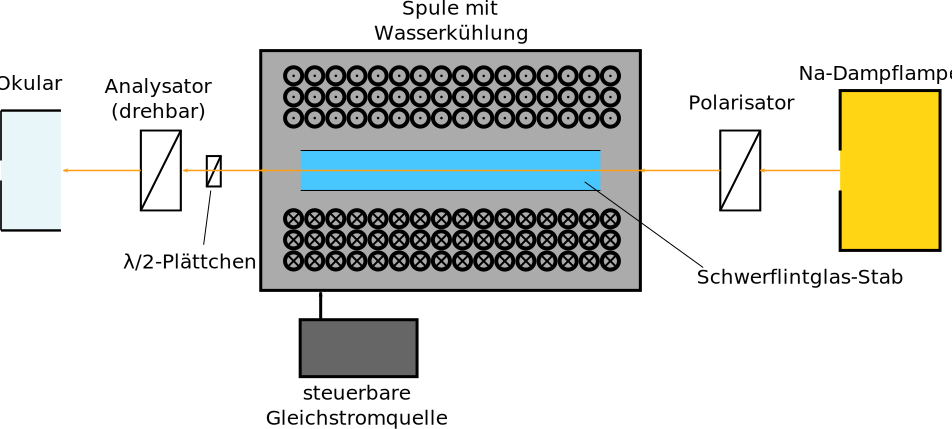
\includegraphics[width=\textwidth]{../img/aufbauFara.pdf}
  \caption{Aufbau zur Messung der Polarisationsdrehung von linear polarisiertem Licht 
  in einem Schwerflintglas-Stab im Magnetfeld einer Spule.}
  \label{img:aufbauFara}
\end{center}
\end{figure}

\autoref{img:aufbauFara} zeigt den Aufbau, der zur Messung des Faraday-Effekts verwendet wird.
Eine Natriumdampflampe liefert monochromatisches Licht ($\lambda_{\text{Na}}\approx$ 589\,nm),
das mit einem Polarisator linear polarisiert wird.
Das polarisierte Licht durchläuft dann einen Stab aus Schwerflintglas,
der sich in einer Spule befindet.
Die Spule ist wassergekühlt und wird durch ein steuerbares Netzteil mit Strom versorgt.
Nach dem Schwerflintglas wird die Polarisationsrichtung eines Teils der Strahlung von einem
\textlambda/2-Plättchen um einen kleinen Winkel gedreht.
Danach fällt der ganze Strahl durch einen drehbaren Analysator.
Diese Konfiguration wird als Halbschattenpolarimeter bezeichnet:
Wenn durch Drehung des Analysators die beiden Teile des Strahls auf gleiche Helligkeit gebracht werden,
zeigt eine Skala den Winkel, um den das Licht im Polarimeter in seiner Polarisation gedreht wird.



\subsection{Versuchsdurchführung}

Am Aufbau für den Faraday-Effekt wird nur eine Messreihe durchgeführt:
Die Drehung der Polarisationsrichtung wird in Abhängigkeit des Spulenstroms $I$
(Variation von -5\,A bis 5\,A in Schritten von 0.5\,A) untersucht.
Jeder Messpunkt wird insgesamt vier mal aufgenommen.
Um eine Drift der Anlage auszuschließen,
werden zuerst die ganzzahligen Messwerte aufgenommen und anschließend die
Zwischenwerte.
Nach der Einstellung des Stroms für jeden Messpunkt wird der Analysator
des Halbschattenpolarimeters so eingestellt, dass die äußeren Strahlteile genauso hell sind wie der innere
Strahlteil.
Es gibt dafür eine helle und eine dunkle Einstellung.
Wegen der logarithmischen Empfindlichkeitskurve des menschlichen Auges wird die dunklere Einstellung
für die Messung verwendet, da daraus eine höhere Messgenauigkeit folgt.

\subsection{Messergebnisse und Auswertung}
\subsubsection{Bestimmung der Verdet-Konstante}
Für jede Spannung $I$ wurde $N=4$ mal der entsprechende Winkel $\alpha_i$ gemessen. Der Fehler einer Einzelmessung des Winkels wurde auf
\begin{equation}
  s_{\alpha_i} = 0.2^\circ
\end{equation}  % TODO Fehler auf Strom
geschätzt. Es wird zunächst der Mittelwert der Winkel gebildet:
\begin{equation}
  \alpha = \frac{1}{N} \sum_{i=1}^{N} \alpha_i, \qquad s_{\alpha} = \frac{s_{\alpha_i}}{\sqrt{N}}
\end{equation}
Der Fehler auf den Strom wurde auf $s_I = 0.1$\,A geschätzt.\\
Die Spannungen und gemittelten Winkel werden nun mit einer Geraden gefittet:
\begin{equation}
  \alpha(I) = a + b \cdot I
\end{equation}
Die Werte und der Fit sind in \autoref{img:faraday} dargestellt. Die Kurvenanpassung ergab folgende Werte:
\begin{equation}
\begin{split}
  \label{eq:faraday:params}
  a &= (-0.28 \pm 0.06)\,{}^\circ \\
  b &= (2.5769 \pm 0.0199)\,\frac{{}^\circ}{\text{A}}
\end{split}
\end{equation}
\begin{figure}[H]
\begin{center}
  \includegraphics[width=\textwidth]{../img/faraday.pdf}
  \caption{Winkel $\alpha$ in Abhängigkeit des Stroms $I$ mit Fit einer Geraden.}
  \label{img:faraday}
\end{center}
\end{figure}
Mit \autoref{eq:verdet} wird nun die Verdet-Konstante $V$ berechnet:
\begin{equation}
  \label{eq:eval:verdet}
  V = \frac{b}{2556}, \qquad s_V = \frac{s_b}{2556}
\end{equation}
\begin{equation}
  V = (1.009 \pm 0.008) \cdot 10^{-3}\,\frac{{}^\circ}{\text{A}}
\end{equation}

\paragraph{Vergleich mit der Herstellerangabe}
Die Verdet-Konstante rechnet man folgendermaßen in $\frac{\text{min}}{\text{Oe}\cdot \text{cm}}$ um:
\begin{equation}
  1\,\frac{{}^\circ}{\text{A}} = \frac{60\cdot 79.58}{100}\,\frac{\text{min}}{\text{Oe}\cdot \text{cm}}
\end{equation}
Es folgt für den berechneten Wert:
\begin{equation}
  V = (0.0482 \pm 0.0004)\,\frac{\text{min}}{\text{Oe}\cdot \text{cm}}
\end{equation}
Der Hersteller gibt:
\begin{equation}
  V^{\text{Herst.}} = 0.05\,\frac{\text{min}}{\text{Oe}\cdot \text{cm}}
\end{equation}
als Wert an. Der gemessene Wert stimmt innerhalb des $5-\sigma$-Intervalls mit der Herstellerangabe überein, vorausgesetzt dass diese keinen Fehler 
besitzt. Betrachtet man die Rundung, so kann die Herstellerangabe zwischen $(0.045 \leq 0.05 < 0.055)\,\frac{\text{min}}{\text{Oe}\cdot \text{cm}}$ liegen. 
Mit diesem Fehler von $0.005\,\frac{\text{min}}{\text{Oe}\cdot \text{cm}}$  würden die beiden Werte innerhalb ihrer Fehler übereinstimmen.

\paragraph{Vergleich mit einer idealen Zylinderspule}
Hätte man anstelle einer realen Zylinderspule eine ideale Spule ($H^{\text{ideal}} = \frac{N \cdot I}{l}$) angenommen, 
so berechnet sich der Drehwinkel nach \autoref{eq:faraday} mit:
\begin{equation}
  \label{eq:alpha:ideal}
  \alpha = V \cdot N \cdot I \quad \Rightarrow b = V \cdot N \Leftrightarrow V = \frac{b}{N}
\end{equation}
Es ergibt sich nun äquivalent zu \autoref{eq:eval:verdet} eine Verdet-Konstante von:
\begin{equation}
  V^{\text{ideal}} = (0.716 \pm 0.006) \cdot 10^{-3}\,\frac{{}^\circ}{\text{A}} = (0.0342 \pm 0.0003)\,\frac{\text{min}}{\text{Oe}\cdot \text{cm}}
\end{equation}
Sie weicht sehr weit von dem Wert der realen Spule und der Herstellerangabe ab, weshalb die Näherung einer idealen Spule nicht gerechtfertigt ist. \\
Des Weiteren sieht man an \autoref{eq:alpha:ideal}, dass die in den Grundlagen (Kapitel \ref{subsub:alpha}) berechnete Konstante 
$c = 2554.85$ eine effektive Windungsanzahl darstellt, die eine ideale Spule besitzen müsste, um das Licht um den gleichen Winkel zu drehen.
\subsubsection{Bestimmung von 2\textepsilon}
Der Winkel $\alpha$ der Stellungen "`innen maximal dunkel"' ($\alpha_i$) und "`außen maximal dunkel"' ($\alpha_a$) wurde 
jeweils $N = 4$ mal gemessen. Der Fehler einer Einzelmessung wurde auf $s_{\alpha_i} = 2^\circ$ geschätzt. 
Es wird der Mittelwert gebildet
\begin{equation}
  \alpha = \frac{1}{N} \sum_{i=1}^{N} \alpha_i, \qquad s_{\alpha} = \frac{s_{\alpha_i}}{\sqrt{N}}
\end{equation}
und die Differenz der beiden Winkel gebildet:\footnote{Die Fehler der beiden Winkel sind gleich ($s_{\alpha_a} = s_{\alpha_b}$), weil hier der 
Messfehler und nicht die Standardabweichung der Messwerte benutzt wurde, da die Standardabweichungen mit dem Fehler $s_\alpha$ übereinstimmen.}
\begin{equation}
  2 \epsilon = \alpha_a - \alpha_i, \qquad s_{2\epsilon} = \sqrt{s_{\alpha_i}^2 + s_{\alpha_a}^2} = \sqrt{2} s_\alpha
\end{equation}
Man erhält für den Winkel $2\epsilon$:
\begin{equation}
  2\epsilon = (11.1 \pm 1.4)^\circ
\end{equation}

\newpage
\bibliographystyle{plain}
\bibliography{refs}

\appendix
\section{Anhang}
\subsection{Messprotokoll}
\includepdf[pages={-}]{../data/protocol.pdf}

\end{document}